\documentclass[11pt]{article}
\usepackage{graphicx}
\usepackage[export]{adjustbox}
\usepackage{float}
\usepackage{amsmath}
\usepackage{siunitx}
\title{Plotting Bode plot with complex roots and zeros with hand }
\date{2018\\ March}
\author{Nail Tosun \\ Electric and Electronic Engineering Departmant, METU}
\begin{document}
\maketitle
\section*{Introduction}
Given second order transfer function can be generalized following form;

\[H(s)=\frac{\omega_n ^2}{s^2+2\xi \omega_n s + \omega_n
}\]

where $\xi$ is \textbf{damping ratio} and $\omega_n$ is natural frequency. 
\paragraph*{}
When $\xi>1$ system response said over-damped, and it can easily separate two first order system cascaded.

Then transfer function rewritten in following form;
\[H(s)=\frac{K}{(s+\alpha)(s+\beta)}\]
Then body plot of that transfer function is straight-forward. 

-Regulate the transfer function 

\[H(s)=\frac{\frac{K}{\alpha \beta}}{(1+\frac{s}{\alpha})(1+\frac{s}{\beta})}\]

-Find the dc-gain (gain at $\omega=0$)
\[G_{dc}=\frac{K}{\alpha \beta}\]

Since there is no zero (no s in the numerator) in the following function also no pole at zero (no zero in the denominator), plot came with straight line before first pole hit.

-Plot the asymptotes and bode

When $\xi=1$ we said system response critically-damped. Denominator can rewrite as $(s+\omega_n)^2$.That means now we have double pole in a particular location. Bode plot algorithm is still same just make sure know we have $40 \frac{dB}{decade}$ 

\section*{Complex poles and zeros}
\subsection*{Complex poles}
All points in second order term with $\xi <1$ is we plot asymptotes like $\xi=1$ case. With closing $\xi$ to one (from zero), transfer function start behave;
\[H(s)=\frac{\omega_n}{(s+\omega_n)^2}\]
The can plot above function bode plot easily. So after that we just should edit a little by looking $\xi$, damping ratio.

\[H(s)=\frac{1}{s^2+2\xi s + 1
}\]

\begin{figure}[H]
  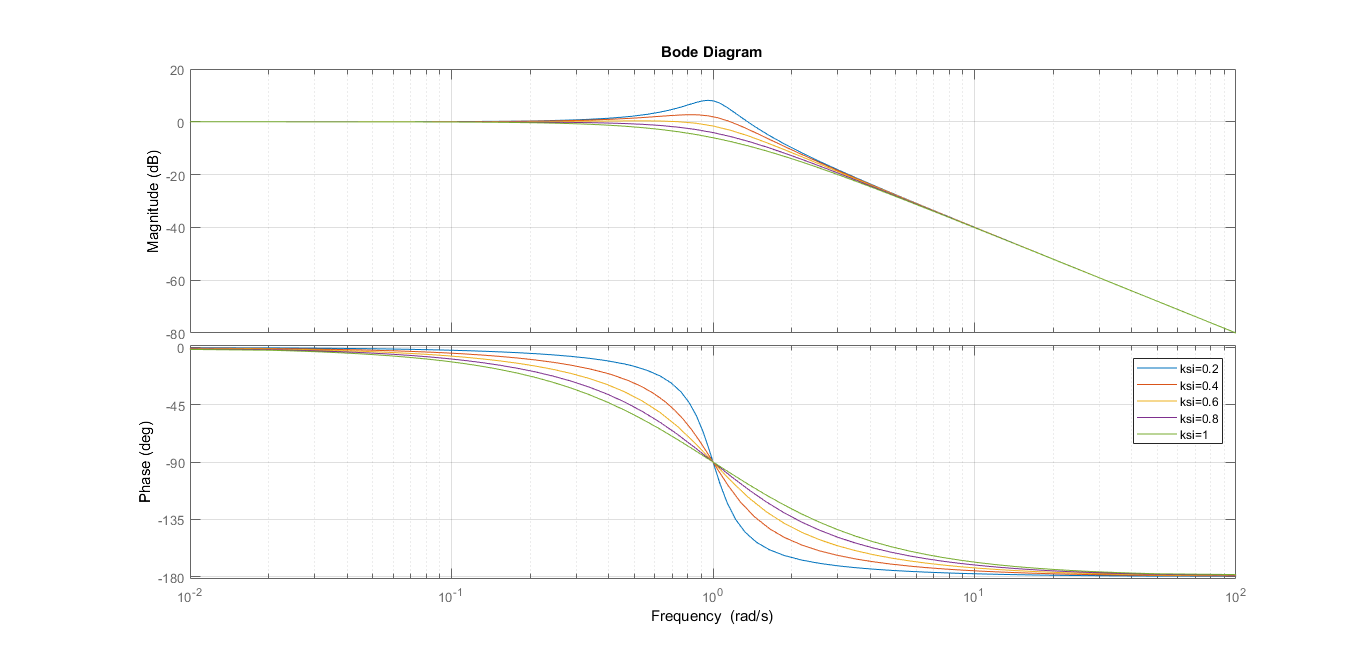
\includegraphics[scale=0.5, center]{complex-poles}
  \caption{Bode plot of H(s) with different $\xi$}
  \label{fig:zero}
\end{figure}

$\xi=1$ , we draw asymptotes and we did -3 dB approximation (for poles). However with $\xi<\frac{1}{\sqrt{2}}$ actual gain underline the other side of the asymptotes (positive over-shoot characteristic for poles). Cut-off frequency also changes slightly with changing $\xi<\frac{1}{\sqrt{2}}$

\[\omega_{n'}=\omega_{n}\sqrt{1-2\xi^2}\]

\section*{Complex zeros}

\[H(s)=s^2+2\xi s + 1\]

\begin{figure}[H]
  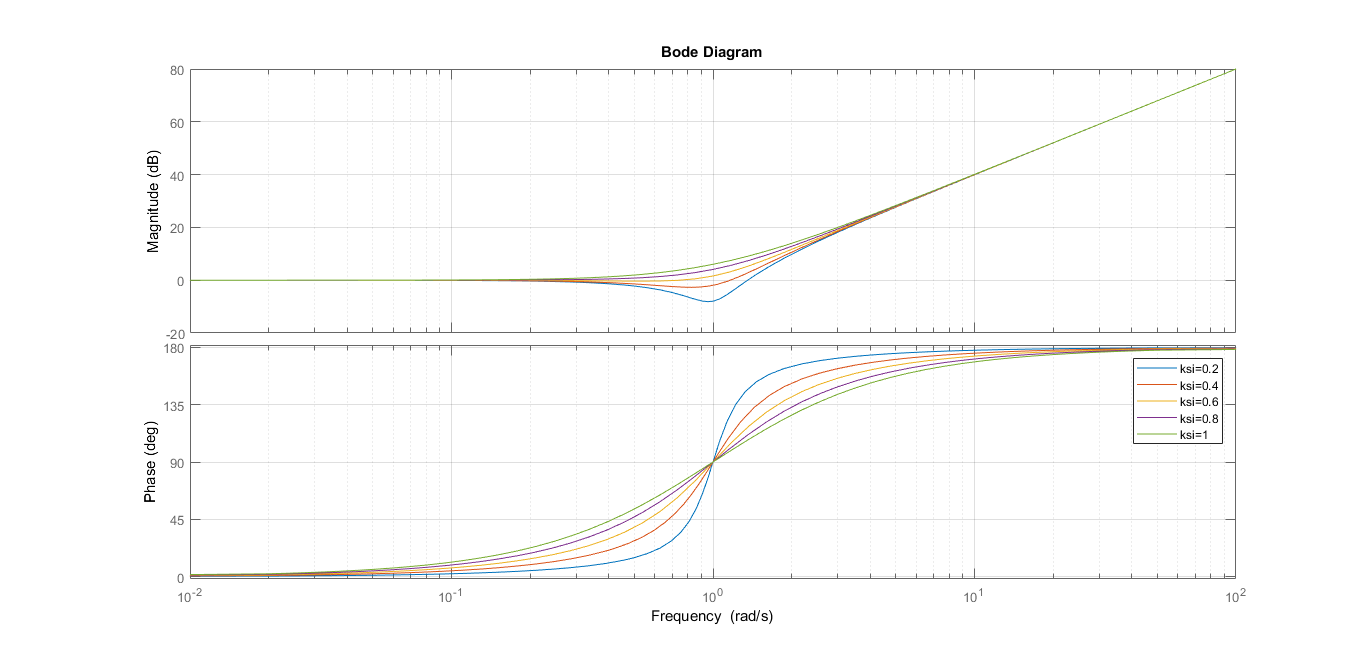
\includegraphics[scale=0.5, center]{complex-zeros}
  \caption{Bode plot of H(s) with different $\xi$}
  \label{fig:zero}
\end{figure}
Similarly, $\xi=1$ , we draw asymptotes and we did +3 dB approximation (for poles). Now the actual gain again is at other side of the asymptote (negative over-shoot characteristic for zeros)

\section*{Example}
\[H(s)=128\frac{s^2+4}{(s+32)(s^2+8s+64)}\]
\subsection*{Behaviour at DC}
System is type-0, no pole at $\omega = 0$ also no zero at $\omega = 0$ therefore straight line comes from the left side of the graph

\subsection*{DC gain}
Normalizing the transfer function;
\[H(s)=\frac{1}{4}\frac{1+\frac{s^2}{4}}{(1+\frac{s}{32})(1+\frac{s}{8}+\frac{s^2}{64})}\]
\[G_{dc}=20log(\frac{1}{4})=-12\> dB\]

\subsection*{Second order Behaviour}
\subsubsection*{Second order pole}
\[s^2+2 \xi \omega_n+ \omega_n^2=s^2+8s+64\]
\[\omega_n=8\]
\[\xi=0.5\]
Double pole at $\omega = 8$
\subsubsection*{Second order zero}
\[s^2+2 \xi \omega_n+ \omega_n^2=s^2+8\]
\[\omega_n=2\]
\[\xi=0\]
Double zero at $\omega=2$

Matlab plot;
\begin{figure}[H]
  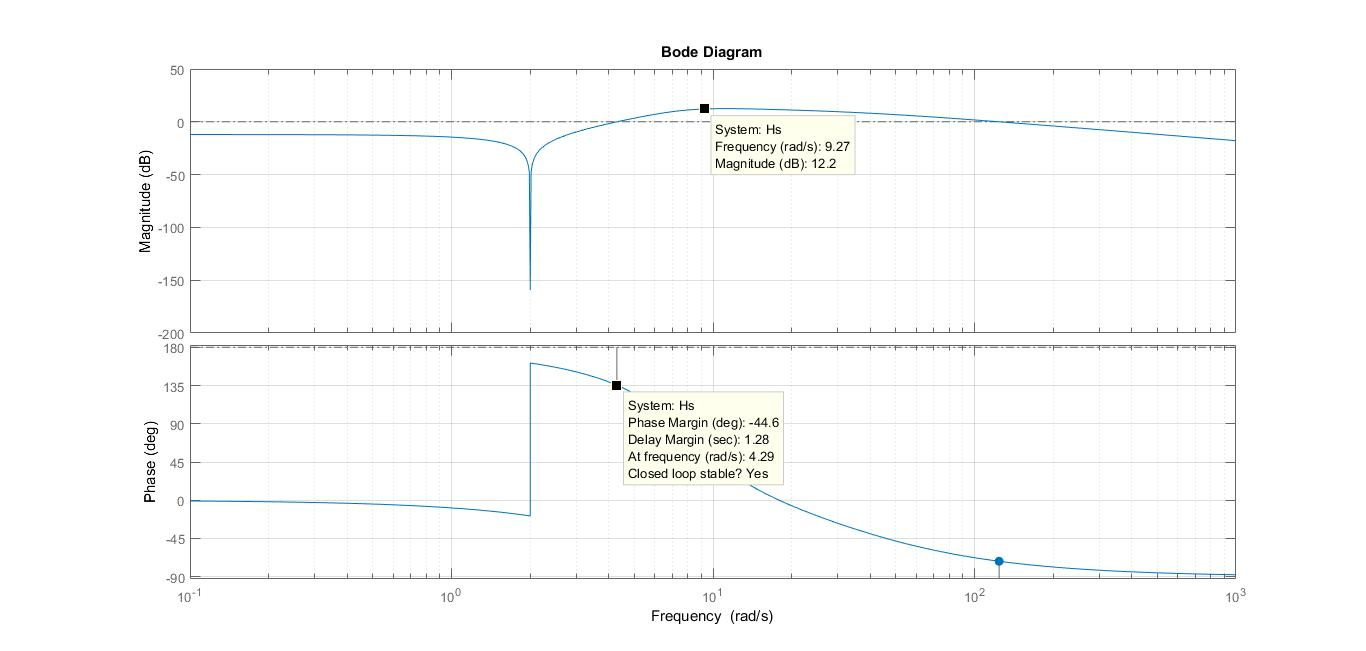
\includegraphics[scale=0.5, center]{sikinti}
  \caption{Bode plot of H(s) with different $\xi$}
  \label{fig:zero}
\end{figure}
By hand;

\end{document}